\chapter{Positivity and the Thorin Toolkit}\label{ch:positivity}

Chapter~\ref{ch:problem} posed the mass gap as a question about the support of a measure. Everything in this book rests on one structural fact: Euclidean correlations of gauge invariant observables are Laplace transforms of nonnegative measures. This chapter explains where the fact comes from, first in the axiomatic setting and then on the lattice, and records the elementary consequences we use throughout (Section~\ref{sec:wherepos}). It then collects the two toolkits used in the rest of the book. Section~\ref{ch:harmonic} gives the harmonic analysis of compact groups (characters, Casimirs, Haar measure, Brownian motion and the Jacobian of the exponential map), which is where positivity takes its group theoretic form. Section~\ref{ch:toolkit} gives the probabilistic toolkit: Stieltjes functions, generalized gamma convolutions and Thorin measures, the hyperbolic laws of Biane, Pitman and Yor, and the orders and inverse problems that the later chapters use. Most of this material is classical, and the reader who knows it may skim.

\section{Where Positivity Comes From}\label{sec:wherepos}

\subsection{Reflection positivity}

Let $\Theta$ denote reflection in the time coordinate, $\Theta(\tau,x)=(-\tau,x)$. For a Euclidean field theory with expectation $\langle\cdot\rangle$, let $\mathcal A_+$ be the algebra of observables supported in the half space $\tau>0$, and let $\Theta$ act on observables in the same way, by reflecting their support and taking complex conjugates. Osterwalder and Schrader\index{Osterwalder, K.!and Schrader, R.}~\cite{OS} showed that a Euclidean theory satisfying the condition
\begin{equation}\label{eq:RP}
\langle\Theta(F)\,F\rangle\ge0\qquad\text{for all }F\in\mathcal A_+,
\end{equation}
together with Euclidean invariance and regularity, can be continued to a relativistic quantum field theory. The construction is concrete. The form $(F,G)=\langle\Theta(F)G\rangle$ is a nonnegative inner product on $\mathcal A_+$. Quotienting by null vectors and completing gives a Hilbert space $\mathcal H$. Time translation by $r\ge0$ maps $\mathcal A_+$ to itself, and its action on $\mathcal H$ is a contraction semigroup of selfadjoint operators $e^{-rH}$ with $H\ge0$. The constant observable $1$ gives the vacuum $\Omega$.

Condition~\eqref{eq:RP} is the source of all positivity in this book. Its content is a positivity statement: the form $\langle\Theta(F)G\rangle$ is a nonnegative inner product, so $\langle\Theta(F)F\rangle\ge0$ for every $F$. It is not by itself a Markov property. For reflections in a plane of sites in a nearest neighbour model there is a stronger structure that implies it: conditioned on the time zero slice, the past and the future are independent and, if the measure is symmetric under $\Theta$, identically distributed after reflection, and then $\langle\Theta(F)F\rangle=\mathbb E\,|\mathbb E[F\mid\text{slice}]|^2\ge0$. This sufficient mechanism is not available for planes that bisect links, where the plaquettes crossing the plane couple past and future; reflection positivity still holds there, as the next subsection shows, but its proof is a different argument.

\subsection{Reflection positivity on the lattice}\label{sec:rplattice}

Osterwalder and Seiler\index{Osterwalder, K.!and Seiler, E.}~\cite{OSe} proved~\eqref{eq:RP} for lattice gauge theory with the Wilson action\index{Wilson action}, for reflections in planes that pass through lattice sites and in planes that bisect links. The argument is short enough to sketch. Write the action as $S=S_++S_-+S_0$, where $S_+$ involves only links in the upper half lattice, $S_-=\Theta S_+$, and $S_0$ collects the plaquettes that cross the reflection plane (for a plane bisecting links; a plane through sites has none). Each crossing plaquette has the form $\operatorname{tr}\big(U\,\Theta(U)^\dagger\big)$ for a product $U$ of upper links. The Boltzmann weight of the crossing plaquettes is a function $f$ of a group element $W=U\Theta(U)^\dagger$, and its character expansion\index{character expansion}
\[
f(W)=\sum_\lambda d_\lambda\,c_\lambda\,\chi_\lambda(W)
\]
has nonnegative coefficients $c_\lambda\ge0$ for the Wilson weight. Since $\chi_\lambda(U\Theta(U)^\dagger)=\sum_{ij}D^\lambda_{ij}(U)\overline{D^\lambda_{ij}(\Theta U)}$, each term is of the form $\Theta(G)G$ summed over matrix elements. Multiplying such terms and integrating against the product Haar measure\index{Haar measure} preserves nonnegativity. The same argument works for any plaquette weight whose character coefficients are nonnegative.

\begin{definition}
A class function $f$ on a compact group $G$ is positive definite if $\sum_{ij}\bar z_if(g_i^{-1}g_j)z_j\ge0$ for all finite families $g_i\in G$, $z_i\in\mathbb C$.
\end{definition}

\begin{proposition}[Bochner on a compact group]\label{prop:bochnergroup}
A continuous class function $f=\sum_\lambda d_\lambda c_\lambda\chi_\lambda$ on a compact group is positive definite if and only if $c_\lambda\ge0$ for every irreducible representation $\lambda$.
\end{proposition}

This is the compact group form of Bochner's theorem~\cite{Bc33}, and it is a classical consequence of the Peter Weyl theorem~\cite{PW27} (Section~\ref{sec:peterweyl}), quoted here without proof. The direction we use most is the easy one: if $c_\lambda\ge0$ then $f$ is positive definite, because each $\chi_\lambda(g_i^{-1}g_j)=\sum_k\langle D^\lambda(g_i)e_k,D^\lambda(g_j)e_k\rangle$ is a Gram matrix in $i,j$. The proposition tells us that the Osterwalder Seiler condition on a plaquette weight is a probabilistic condition: the weight, normalised, is the law of a random group element whose Fourier coefficients are nonnegative. We return to this in Section~\ref{ch:mk}, where every rung of a renormalization ladder will turn out to satisfy it.

L\"uscher~\cite{Lu77} completed the picture by constructing, for the Wilson action, a selfadjoint and strictly positive transfer matrix\index{transfer matrix} $\mathcal T$ on the space of gauge invariant functions of the spatial links. One lattice time step is multiplication by $\mathcal T=e^{-aH}$, normalised so that the vacuum eigenvalue is $1$ and $\|\mathcal T\|=1$, which defines the lattice Hamiltonian $H\ge0$.

Reflection positivity has a concrete matrix form. For times $\tau_i=i\delta$, the Hankel matrix $C(\tau_i+\tau_j)$ of a reflection positive correlation is positive semidefinite, because it is the Gram matrix of the states $e^{-\tau_iH}O\Omega$. Figure~\ref{fig:rphankel} contrasts a sum of three exponentials, whose Hankel matrix has three positive eigenvalues and the rest zero, with a damped cosine, which has the right decay but is not reflection positive and has a negative eigenvalue.

\begin{figure}[t]
\centering
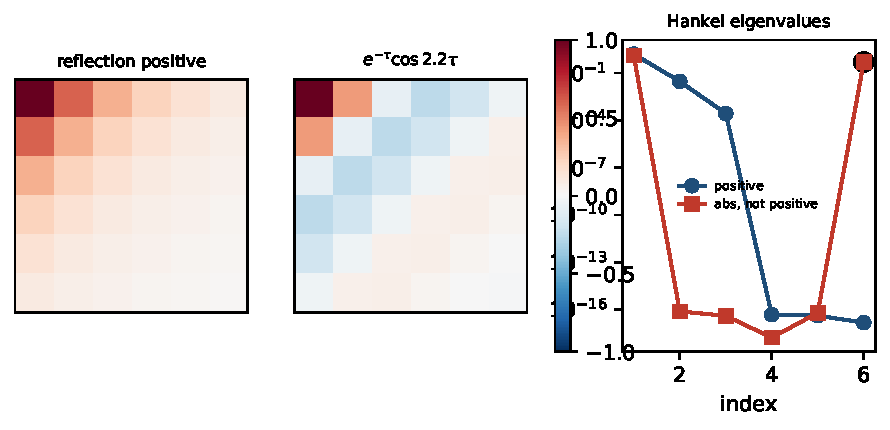
\includegraphics[width=0.95\textwidth]{figures/rp_hankel.pdf}
\caption[Reflection positivity as a Hankel condition]{Hankel matrices $C(\tau_i+\tau_j)$ on a grid of six times for a reflection positive correlation (left) and for $e^{-\tau}\cos2.2\tau$ (centre), and the absolute values of their eigenvalues (right); circled points are negative eigenvalues.}
\label{fig:rphankel}
\end{figure}

\subsection{Bernstein's theorem and the spectral measure}\label{sec:bernstein}

Fix a gauge invariant observable $O$ at zero spatial momentum and remove its vacuum expectation (we assume a unique vacuum). Then
\[
C(\tau)=\langle O,e^{-\tau H}O\rangle=\int_{(0,\infty)}e^{-\tau E}\mu(\mathrm dE),
\]
where $\mu(A)=\|P_A\,O\Omega\|^2$ for the spectral projections $P_A$ of $H$. In particular $C$ is completely monotone:
\[
(-1)^kC^{(k)}(\tau)=\int E^ke^{-\tau E}\mu(\mathrm dE)\ge0 .
\]
Conversely, Bernstein\index{Bernstein theorem}'s theorem~\cite{Be29} (see Widder's treatise on the Laplace transform~\cite{Wi41}) says that every completely monotone function on $(0,\infty)$ is the Laplace transform of a unique nonnegative measure. Complete monotonicity of the Euclidean correlation is therefore exactly equivalent to the existence of a nonnegative spectral measure\index{spectral measure}.

\begin{definition}
The gap of $O$ is $\Delta_O=\inf\operatorname{supp}\mu$. The gap of the theory is $\Delta=\inf_O\Delta_O$, the infimum over gauge invariant observables.
\end{definition}

On the lattice in finite volume, $\tau$ runs over multiples of $a$ and $C(na)=\sum_kc_k\lambda_k^n$ is a mixture of powers of the transfer matrix eigenvalues $\lambda_k=e^{-aE_k}\in(0,1)$. In the continuum $\mu$ can have atoms, the stable glueball\index{glueball}s, and a continuous part, the multiparticle states above threshold.

\subsection{The offset measure}\label{sec:offset}

For composite operators in four dimensions, $C(\tau)$ is singular at $\tau=0$. For $\operatorname{tr}F^2$ at zero momentum it grows like $\tau^{-5}$, so $\mu$ has infinite mass and quantities such as $\int_0^\infty C$ diverge. We avoid this by working at a positive Euclidean time.

\begin{definition}
For $\alpha>0$ such that $C(\alpha)<\infty$, the offset measure is $\mu_\alpha(\mathrm dE)=e^{-\alpha E}\mu(\mathrm dE)$, and the offset correlation is $C(\alpha+\tau)=\int e^{-\tau E}\mu_\alpha(\mathrm dE)$.
\end{definition}

The offset multiplies $\mu$ by a strictly positive function, so it leaves the support, and hence the gap, unchanged. It plays the same role as smearing the operator in time, or applying gradient flow at a positive flow time. Throughout, $\alpha_0$ denotes a time with $C(\alpha_0)<\infty$, and offsets are taken with $\alpha>\alpha_0$.

\subsection{First consequences}\label{sec:first}

Three elementary facts follow from positivity and are used repeatedly.

\begin{proposition}[log convexity]\label{prop:logconvex}
For $\mu\ne0$, on $\tau>\alpha_0$ (where $C$ is finite), $\tau\mapsto\log C(\tau)$ is convex. Hence the effective mass $m_{\mathrm{eff}}(\tau)=-\frac{\mathrm d}{\mathrm d\tau}\log C(\tau)$ is nonincreasing, and $m_{\mathrm{eff}}(\tau)\downarrow\Delta_O$ as $\tau\to\infty$.
\end{proposition}

\begin{proof}
For $\tau=\frac12(\tau_1+\tau_2)$, Cauchy and Schwarz give $C(\tau)^2\le C(\tau_1)C(\tau_2)$. The limit follows from Laplace's method applied to $\int e^{-\tau E}\mu(\mathrm dE)$.
\end{proof}

The proposition has a sharp methodological consequence. For the exact correlator every effective mass is an upper bound on the gap, and estimates from noisy data inherit this only up to statistical error. Numerical work can show that a claimed gap is too large, but it can never certify that a gap exists. A proof of a gap must come from analysis of the transfer matrix itself.

\begin{proposition}[mixture of exponentials]\label{prop:mixexp}
If $\int_0^\infty C(\alpha+s)\,\mathrm ds<\infty$, as when $\Delta_O>0$, the normalised offset correlation $p(\tau)=C(\alpha+\tau)/\int_0^\infty C(\alpha+s)\mathrm ds$ is a probability density on $(0,\infty)$ that is a mixture of exponential densities, with mixing measure proportional to $\mu_\alpha(\mathrm dE)/E$. By the theorem of Goldie and Steutel~\cite{Go67,St67} it is infinitely divisible.
\end{proposition}

The first two assertions are a one line computation: $p(\tau)=Z^{-1}\int Ee^{-\tau E}\,\mu_\alpha(\mathrm dE)/E$ with $Z=\int\mu_\alpha(\mathrm dE)/E=\int_0^\infty C(\alpha+s)\mathrm ds$, and $Ee^{-\tau E}$ is the exponential density with rate $E$. The infinite divisibility of exponential mixtures is the classical theorem of Goldie and Steutel, which we quote without proof.

\begin{proposition}[gap and decay]\label{prop:gapdecay}
$\Delta_O\ge m$ if and only if there is a constant $K$ with $C(\tau)\le Ke^{-m\tau}$ for all large $\tau$.
\end{proposition}

\begin{proof}
If the support is in $[m,\infty)$, then $C(\tau)\le e^{-m(\tau-\alpha_0)}C(\alpha_0)$. Conversely, if $\Delta_O<m$, a dyadic cover of $[\Delta_O,m)$ gives $\varepsilon>0$ with $\mu([m-2\varepsilon,m-\varepsilon])=c>0$, and then then $C(\tau)\ge c\,e^{-(m-\varepsilon)\tau}$, which eventually exceeds $Ke^{-m\tau}$.
\end{proof}

\subsection{Two examples}\label{sec:examples}

\begin{example}[the Wilson plaquette for SU(2)]
For SU(2) the Wilson weight of a plaquette with rotation angle $\theta$ is $e^{\beta\cos\theta}$. Its character coefficients, normalised by the trivial one, are
\[
u_n(\beta)=\frac{I_n(\beta)}{I_1(\beta)},\qquad n=1,2,3,\dots,
\]
where $n$ is the dimension of the representation and $I_\nu$ is the modified Bessel function. All are positive, and $u_2(\beta)\sim\beta/4$ as $\beta\to0$, while $u_n(\beta)\approx\exp(-(n^2-1)/(2\beta))$ as $\beta\to\infty$.
\end{example}

\begin{example}[the heat kernel plaquette]
The heat kernel\index{heat kernel} action has $u_n=e^{-t(n^2-1)/4}$ for a parameter $t>0$. At weak coupling it matches the Wilson action with $t=2/\beta$. As Section~\ref{sec:bmgroup} shows, it is the law of Brownian motion\index{Brownian motion on SU(2)} on SU(2) run for time $t$, and its coefficients multiply under convolution. This makes it the natural plaquette weight for renormalization.
\end{example}

The rest of the book takes positivity for granted and asks the other question: where do the measures live? The next two sections supply the tools for that question.

\section{Harmonic Analysis on Compact Groups}\label{ch:harmonic}

The two and four dimensional chapters (Chapters~\ref{ch:twod} and~\ref{ch:strong}) compute with characters, Casimir\index{Casimir}s, heat kernel\index{heat kernel}s and Haar measure\index{Haar measure} on SU(2) and SU(3). This section collects the facts we need, with an emphasis on the probabilistic objects: Brownian motion\index{Brownian motion on SU(2)} on a compact group, its law, and the Jacobian of the exponential map.

\subsection{The Peter Weyl theorem}\label{sec:peterweyl}

Let $G$ be a compact Lie group with Haar probability measure. The Peter Weyl theorem says that the matrix entries of the irreducible unitary representations form an orthogonal basis of $L^2(G)$, and that the characters $\chi_\lambda$ form an orthonormal basis of the class functions. Every square integrable class function has a convergent expansion $f=\sum_\lambda d_\lambda c_\lambda\chi_\lambda$, and Parseval reads $\int|f|^2=\sum_\lambda d_\lambda^2|c_\lambda|^2$.

The characters are positive definite functions, and Proposition~\ref{prop:bochnergroup} says that a class function is positive definite if and only if its coefficients are nonnegative.

\subsection{Maximal tori and the Weyl integration formula}\label{sec:weylint}

Every element of SU(N) is conjugate to a diagonal matrix $\operatorname{diag}(e^{i\theta_1},\dots,e^{i\theta_N})$ with $\sum\theta_j\equiv0\pmod{2\pi}$, unique up to permutation of the angles. A class function is therefore a symmetric function on the maximal torus. The Weyl integration formula expresses Haar integrals of class functions as torus integrals:
\[
\int_{\SU(N)}f(U)\,\mathrm dU=\frac{1}{N!}\int_{T}f(\theta)\,|V(\theta)|^2\,\mathrm d\theta,\qquad V(\theta)=\prod_{j<k}\big(e^{i\theta_j}-e^{i\theta_k}\big),
\]
with $\mathrm d\theta$ the normalised measure on the torus. For SU(2), with $\theta_1=-\theta_2=\theta$, this gives $|V|^2=4\sin^2\theta$ and the density $\frac2\pi\sin^2\theta$ on $[0,\pi]$ used throughout.

The factor $|V|^2$ is the probabilistic signature of the group: it is the Jacobian of the map from the torus times the flag manifold to the group, and it vanishes when eigenvalues collide. The eigenvalues of a Haar random unitary matrix repel each other, which is the starting point of random matrix theory.

\subsection{The Weyl character formula}\label{sec:weylchar}

Irreducible representations of SU(N) are labelled by highest weights, equivalently by partitions $\lambda_1\ge\lambda_2\ge\dots\ge\lambda_N=0$. Their characters are ratios of alternants:
\[
\chi_\lambda(\theta)=\frac{\det\big[e^{i(\lambda_j+N-j)\theta_k}\big]}{\det\big[e^{i(N-j)\theta_k}\big]}.
\]
For SU(2) this gives $\chi_n(\theta)=\sin n\theta/\sin\theta$ with $n=\lambda_1+1$ the dimension. For SU(3), labelling representations by Dynkin indices $(p,q)$, the dimension is $\frac12(p+1)(q+1)(p+q+2)$ and the quadratic Casimir is
\[
C_2(p,q)=\tfrac13\big(p^2+q^2+pq+3p+3q\big),
\]
so the fundamental representation has dimension $3$ and Casimir $4/3$. These formulas drive the SU(3) computation of Section~\ref{ch:mk}, where class functions are represented on a grid on the two dimensional torus and characters are evaluated from the Weyl formula.

\subsection{Casimirs and the Laplacian}\label{sec:casimir}

The Laplace Beltrami operator of a biinvariant metric on $G$ acts on each matrix entry of the representation $\lambda$ as multiplication by $-C_2(\lambda)$, up to a normalisation of the metric. In particular each character is an eigenfunction. For SU(2) in the normalisation of this book the eigenvalues are $(n^2-1)/4$, and the smallest nonzero one is $3/4$. For SU(N) the gap of the Laplacian is the Casimir of the fundamental representation, $(N^2-1)/(2N)$ in the standard normalisation.

\subsection{Brownian motion on a compact group}\label{sec:bmgroup}

Brownian motion on $G$ is the diffusion generated by the Laplacian, in the normalisation fixed by $K_t$ below. It is a L\'evy process on the group: its increments over disjoint time intervals are independent, and their laws are invariant under conjugation. Its law at time $t$, started from the identity, has density with respect to Haar measure
\[
K_t(U)=\sum_\lambda d_\lambda\,e^{-tC_2(\lambda)}\chi_\lambda(U),
\]
a class function with nonnegative coefficients $e^{-tC_2(\lambda)}$. The family $\{K_t\}$ is a convolution semigroup: $K_t*K_s=K_{t+s}$. Its Fourier coefficients $u_\lambda(t)=e^{-tC_2(\lambda)}$ are exponentials, and the Casimir $C_2(\lambda)$ is the rate at which the $\lambda$ coefficient decays.

Three facts about $K_t$ recur.
\begin{enumerate}
\item[(i)] As $t\to\infty$, $K_t\to1$, the Haar density, at the exponential rate set by the smallest nonzero Casimir.
\item[(ii)] As $t\to0$, $K_t$ concentrates at the identity. Near the identity the group looks like its Lie algebra, and $K_t$ is approximately a Gaussian density on $\mathfrak g$ with covariance proportional to $t$, multiplied by the Jacobian correction of the next section.
\item[(iii)] For SU(2), Poisson resummation gives the exact image formula of Section~\ref{sec:su2bm}, which expresses $K_t$ as a sum over geodesics from the identity to $U$.
\end{enumerate}

\subsection{The Jacobian of the exponential map}\label{sec:jacobian}

The exponential map $\exp:\mathfrak g\to G$ is a diffeomorphism from a neighbourhood of zero onto a neighbourhood of the identity. On class functions, written in terms of a Cartan element $X$, the Haar measure pulled back to $\mathfrak g$ has density
\[
j(X)=\prod_{\alpha>0}\Big(\frac{\sin(\alpha(X)/2)}{\alpha(X)/2}\Big)^2
\]
with respect to Lebesgue measure, where $\alpha$ runs over the positive roots. For SU(2) the single positive root gives $j=(\sin\theta/\theta)^2$. The heat kernel near the identity has the classical expansion
\[
K_t(\exp X)\approx(4\pi t)^{-\dim G/2}\,j(X)^{-1/2}\,e^{-|X|^2/(4t)}\,e^{t\,\rho^2},
\]
where $\rho$ is half the sum of the positive roots and the constant depends on normalisation. The factor $j^{-1/2}=\prod_{\alpha>0}\frac{\alpha(X)/2}{\sin(\alpha(X)/2)}$ is exactly the curvature factor of Section~\ref{ch:mk}. For SU(2) it is $\theta/\sin\theta$, and for SU(N) it is the product over the $N(N-1)/2$ pairs $p<q$ of $\frac{(\theta_p-\theta_q)/2}{\sin((\theta_p-\theta_q)/2)}$.

\subsection{Curvature factors as Laplace transforms}\label{sec:curvature}

At imaginary argument each root factor becomes $x/\sinh x$, and
\[
\frac{x}{\sinh x}=\prod_{n\ge1}\Big(1+\frac{x^2}{\pi^2n^2}\Big)^{-1}=\E\exp\Big(-\frac{x^2}{2}S_{\mathrm{BPY}}\Big),
\]
where $S_{\mathrm{BPY}}$ is the Biane Pitman Yor\index{Biane Pitman Yor variable} variable of Section~\ref{sec:bpy}, a generalized gamma convolution\index{generalized gamma convolution} with Thorin atoms at $\pi^2n^2/2$. The curvature factor of SU(N) at imaginary angle is therefore the Laplace transform of a weighted sum of $N(N-1)/2$ independent copies of $S_{\mathrm{BPY}}$. Its logarithm to second order is minus the mean, $\E S_{\mathrm{BPY}}=1/3$, times a quadratic form in the angles. That single number, multiplied by the number of positive roots and the root normalisation, will turn out, with the scale factors of the recursion, to give the coefficient of asymptotic freedom\index{asymptotic freedom} in the Migdal Kadanoff\index{Migdal Kadanoff recursion} approximation.

\subsection{Positive definiteness under products}\label{sec:pdprod}

Finally, the fact that makes the Migdal Kadanoff ladder positivity preserving. If $f$ and $g$ are class functions with nonnegative character coefficients, then so is $fg$, because
\[
\chi_\mu\chi_\nu=\sum_\lambda N^\lambda_{\mu\nu}\chi_\lambda,\qquad N^\lambda_{\mu\nu}\in\{0,1,2,\dots\}.
\]
For SU(2) the multiplicities are all zero or one, and the rule is the Clebsch Gordan\index{Clebsch Gordan rule} series $\chi_m\chi_n=\chi_{|m-n|+1}+\chi_{|m-n|+3}+\dots+\chi_{m+n-1}$. For SU(3) multiplicities greater than one occur, but they are still nonnegative integers. Positive definite functions on a compact group therefore form a cone closed under both pointwise multiplication and convolution, the two operations of renormalization.

\section{The Probabilistic Toolkit}\label{ch:toolkit}

The probabilistic objects used in the rest of the book come next. Their arrangement reflects our Riemann programme~\cite{PS26a}, where they were assembled for a different purpose.

\subsection{Laplace transforms and Stieltjes functions}\label{sec:stieltjes}

For a nonnegative measure $\nu$ on $[0,\infty)$ write $\hat\nu(s)=\int e^{-sx}\nu(\mathrm dx)$. A function $g$ on $(0,\infty)$ is a Stieltjes function\index{Stieltjes function} if
\[
g(s)=a+\int_{[0,\infty)}\frac{\sigma(\mathrm dt)}{s+t}
\]
for some $a\ge0$ and a nonnegative measure $\sigma$ with $\int(1+t)^{-1}\sigma(\mathrm dt)<\infty$. A Stieltjes function extends analytically to $\mathbb C\setminus(-\infty,0]$, and the measure is recovered from the jump across the cut:
\[
\sigma(\mathrm dt)=\lim_{\varepsilon\downarrow0}\frac{1}{\pi}\operatorname{Im}g(-t-i\varepsilon)\,\mathrm dt
\]
in the weak sense. This Stieltjes inversion formula is the main analytic tool in Chapter~\ref{ch:routeA}. The Laplace transform of a completely monotone function that is integrable near $0$, such as an offset correlation, is a Stieltjes function: if $C(\tau)=\int e^{-\tau E}\mu(\mathrm dE)$ then $\int_0^\infty e^{-s\tau}C(\tau)\mathrm d\tau=\int\mu(\mathrm dE)/(s+E)$.

\subsection{Generalized gamma convolutions}\label{sec:ggc}

The gamma law with shape $a$ and rate $t$ has Laplace transform $(1+s/t)^{-a}$. A finite convolution of gamma laws with shapes $a_j$ and rates $t_j$ has Laplace transform $\exp(-\sum_ja_j\log(1+s/t_j))$. Thorin, studying the infinite divisibility of the Pareto and log normal laws in 1977~\cite{Th77,Th77b}, introduced the closure of this class under weak limits.

\begin{definition}
A probability law on $[0,\infty)$ is a generalized gamma convolution\index{generalized gamma convolution} (GGC) if its Laplace transform has the form
\[
\varphi(s)=\exp\Big(-a s-\int_{(0,\infty)}\log\big(1+\tfrac st\big)U(\mathrm dt)\Big),
\]
with $a\ge0$ and a nonnegative measure $U$, the Thorin measure\index{Thorin measure}, satisfying $\int_{(0,1]}|\log t|\,U(\mathrm dt)<\infty$ and $\int_{(1,\infty)}t^{-1}U(\mathrm dt)<\infty$.
\end{definition}

Differentiating,
\[
-\frac{\mathrm d}{\mathrm ds}\log\varphi(s)=a+\int\frac{U(\mathrm dt)}{s+t},
\]
so a law is a GGC exactly when the logarithmic derivative of its Laplace transform is a Stieltjes function. This characterisation is what Chapter~\ref{ch:routeA} uses. Bondesson\index{Bondesson, L.}'s monograph~\cite{Bo92} develops the theory; we record the facts we need, with their proofs left to that source.

\begin{proposition}[properties of GGC, quoted from~\cite{Bo92}]\label{prop:ggcprops}
\begin{enumerate}
\item[(i)] The class is closed under convolution and under weak limits. Under weak convergence the Thorin measures converge vaguely.
\item[(ii)] Every GGC is infinitely divisible and self decomposable. Its L\'evy measure has density $k(x)/x$ with $k(x)=\int e^{-xt}U(\mathrm dt)$ completely monotone.
\item[(iii)] (Bondesson) A GGC with $a=0$ is the law of $\sum_jY_j/T_j$, where $(T_j,Y_j)$ are the points of a Poisson process on $(0,\infty)^2$ with intensity $U(\mathrm dt)\,y^{-1}e^{-y}\mathrm dy$: a shot noise of the jumps of a gamma process, rescaled by rates drawn from the Thorin measure. When $U$ has atoms of integer mass the gamma jumps can be replaced by exponential variables, as for $S_{\mathrm{BPY}}$ below.
\item[(iv)] A law with density $f$ is hyperbolically completely monotone (HCM) if $f(uv)f(u/v)$ is completely monotone in $v+1/v$ for each $u>0$. Every HCM law is a GGC.
\end{enumerate}
\end{proposition}

Part (iii) gives the probabilistic meaning of the Thorin measure: it is the intensity of the rates in a shot noise. The left edge of its support is the slowest available rate, and it sets the exponential tail of the law. Chapter~\ref{ch:routeA} uses exactly this.

\subsection{L\'evy measures and compound Poisson processes}\label{sec:levy}

A L\'evy process $X$ on $\R$ with symmetric L\'evy measure and no Gaussian part has characteristic function $\E e^{itX_1}=e^{-\psi(t)}$ with
\[
\psi(t)=\int_{\R}\big(1-\cos tx\big)\,\nu(\mathrm dx).
\]
When $\nu$ is finite, $X$ is a compound Poisson process: jumps arrive at rate $\nu(\R)$ and have law $\nu/\nu(\R)$. If $\nu$ lives on $(0,\infty)$ we symmetrise it, so that $\psi(t)=\int_{(0,\infty)}(1-\cos tx)\nu(\mathrm dx)$. Section~\ref{ch:routeB} will show that the Thorin densities produced by the $2\sin^2$ lemma are exactly such L\'evy exponent\index{Levy exponent@L\'evy exponent}s, divided by $\pi t$.

\subsection{The hyperbolic laws of Biane, Pitman and Yor}\label{sec:bpy}

Biane, Pitman and Yor~\cite{BPY} studied a family of laws attached to Brownian motion\index{Brownian motion on SU(2)} and Bessel processes whose Laplace transforms are hyperbolic functions:
\[
\E e^{-\lambda C}=\frac{1}{\cosh\sqrt{2\lambda}},\qquad
\E e^{-\lambda S_{\mathrm{BPY}}}=\frac{\sqrt{2\lambda}}{\sinh\sqrt{2\lambda}},\qquad
\E e^{-\lambda T}=\frac{\tanh\sqrt{2\lambda}}{\sqrt{2\lambda}} .
\]
The variable $C$ is the first exit time of Brownian motion from $(-1,1)$. The variable $S_{\mathrm{BPY}}$ is the first hitting time of $1$ by a three dimensional Bessel process started at $0$. These laws are tied to the Jacobi theta function, and through it to the Riemann zeta function; Biane, Pitman and Yor show that the Riemann $\xi$ function appears as a Mellin transform of a closely related law. The infinite product expansions of $\cosh$ and $\sinh$ give, for example,
\[
\frac{\sqrt{2\lambda}}{\sinh\sqrt{2\lambda}}=\prod_{n\ge1}\Big(1+\frac{2\lambda}{\pi^2n^2}\Big)^{-1},
\]
so $S_{\mathrm{BPY}}$ is a GGC with Thorin measure $\sum_n\delta_{\pi^2n^2/2}$: an infinite sum of independent exponential variables with rates $\pi^2n^2/2$. Its mean is
\[
\E S_{\mathrm{BPY}}=\sum_{n\ge1}\frac{2}{\pi^2n^2}=\frac13 .
\]
Similarly $\E C=1$ and $\E T=2/3$.

\begin{figure}[t]
\centering
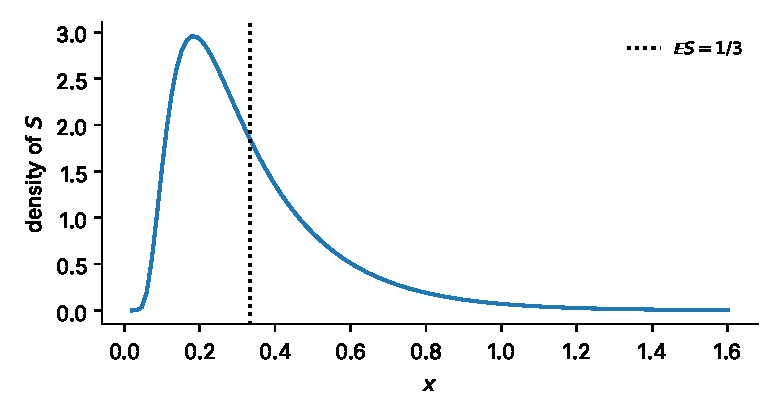
\includegraphics[width=0.92\textwidth]{figures/bpy_density.pdf}
\caption[The density of the Biane Pitman Yor variable $S_{\mathrm{BPY}}$]{The density of the Biane Pitman Yor variable $S_{\mathrm{BPY}}$, computed by numerical inversion of $\sqrt{2\lambda}/\sinh\sqrt{2\lambda}$. Its mean $1/3$ enters the coefficient of asymptotic freedom in the Migdal Kadanoff approximation of Section~\ref{ch:mk}.}
\label{fig:bpy}
\end{figure}

The P\'olya Gamma\index{Polya Gamma@P\'olya Gamma} laws of Polson, Scott and Windle~\cite{PSW13} belong to the same family. The variable $\mathrm{PG}(b,0)$ has Laplace transform $\cosh^{-b}\sqrt{\lambda/2}$, so $\mathrm{PG}(b,0)$ has the law of $C_b/4$, where $C_b$ is the sum of $b$ independent copies of $C$. The exponential tilting $\mathrm{PG}(b,c)$ is what makes Gibbs sampling for logistic models conjugate. The variable $S_{\mathrm{BPY}}$ appears in this book for a different reason, explained in Section~\ref{sec:curvature}: the inverse square root $\theta/\sin\theta$ of the Jacobian of the exponential map of SU(2), continued to imaginary angle, is its Laplace transform.

\subsection{Products and convolutions}\label{sec:prodconv}

Two operations on probability laws recur in renormalization. Given densities $f$ and $g$ with respect to a common reference measure, the normalised product $fg/\int fg$ is the posterior obtained by combining two independent pieces of evidence, and the $k$th normalised power $f^k/\int f^k$ is the posterior from $k$ independent copies of the likelihood $f$. The convolution $f*g$ is the law of a sum of independent variables, or of a product of independent group elements.

For Gaussian laws on $\R^m$ the two operations are dual in the simplest possible way:
\[
\text{product: precisions add},\qquad\text{convolution: variances add}.
\]
Polson and Scott~\cite{PSdual} develop this duality, between mixtures (convolutions) and envelopes (products), as a general principle of hierarchical modelling. In Section~\ref{ch:mk} it becomes the bookkeeping of the Migdal Kadanoff\index{Migdal Kadanoff recursion} recursion, and the failure of exact duality on a curved group is what drives asymptotic freedom\index{asymptotic freedom} in that approximation.

\subsection{Likelihood ratio orders}\label{sec:lro}

\begin{definition}
A family of densities $\{f_t\}$ on an interval has monotone likelihood ratio\index{likelihood ratio order} in $t$ if $f_{t'}(x)/f_t(x)$ is increasing in $x$ whenever $t'>t$. Equivalently, for smooth positive densities, $\partial_x\log f_t(x)$ is increasing in $t$.
\end{definition}

\begin{proposition}\label{prop:lro}
\begin{enumerate}
\item[(i)] If $\{f_t\}$ has monotone likelihood ratio, then $f_{t'}$ is stochastically larger than $f_t$ for $t'>t$, so $\int h\,f_t$ is increasing in $t$ for every increasing $h$.
\item[(ii)] Monotone likelihood ratio is preserved by normalised products with a fixed positive function, and by taking powers.
\item[(iii)] (Karlin~\cite{Ka68}) Monotone likelihood ratio is preserved by convolution with a log concave density.
\end{enumerate}
\end{proposition}

Parts (i) and (iii) are classical, and we quote them from Karlin~\cite{Ka68} without proof; part (ii) is immediate, since multiplying by a fixed positive function leaves the ratio $f_{t'}/f_t$ unchanged and powers preserve monotonicity of a positive ratio. Part (iii) is a statement about total positivity of order two; log concave densities are P\'olya frequency functions of order two, and the composition of totally positive kernels is totally positive. Section~\ref{ch:verification} uses (i) and (ii) to prove that a renormalization map is monotone. Chapter~\ref{ch:path} asks whether (iii) can survive on a curved group, where the relevant kernels are no longer log concave.

\subsection{Positive linear inverse problems}\label{sec:pliv}

Finally, recovering a nonnegative measure $\mu$ from noisy observations of a linear functional $K\mu$ is a positive linear inverse problem. Vardi and Lee\index{Vardi, Y.!and Lee, D.}~\cite{VL} gave the EM algorithm
\[
\nu^{(r+1)}=\nu^{(r)}\cdot\frac{K^\top\big(y/K\nu^{(r)}\big)}{K^\top 1},
\]
which preserves positivity and decreases a Kullback Leibler divergence (that is, increases the likelihood). Polson and Robert~\cite{PR}, in their discussion of Vardi and Lee, interpreted the inversion as a von Neumann style Monte Carlo procedure. Padilla, Polson and Scott~\cite{PPS} give Bayesian nonparametric deconvolution with theoretical guarantees, and Polson, Scott and Willard~\cite{PSW15} survey the proximal algorithms that accelerate such schemes. Chapter~\ref{ch:estimation} applies these ideas to the inverse Laplace problem of extracting a spectrum from a correlator, where the support edge, and so the gap, is far better determined than the measure itself.

\section*{Exercises}
\begin{enumerate}
\item (Section~\ref{sec:examples}) Show directly that the Wilson weight $e^{\beta\cos\theta}$ on SU(2) has positive character coefficients $u_n=I_n(\beta)/I_1(\beta)$, using the generating function $e^{\beta\cos\theta}=\sum_{m\in\Z}I_m(\beta)e^{im\theta}$ and $\chi_n(\theta)\sin\theta=\sin n\theta$.
\item (Section~\ref{sec:first}) Prove that a mixture of exponential densities is log convex, and deduce the monotonicity of the effective mass in Proposition~\ref{prop:logconvex} without using the spectral theorem.
\item (Section~\ref{sec:first}) Let $C(\tau)=\sum_{k=1}^Kc_ke^{-E_k\tau}$ with $c_k>0$ and $0<E_1<\dots<E_K$. Compute $m_{\mathrm{eff}}(\tau)$ and show that $m_{\mathrm{eff}}(\tau)-E_1$ decays like $e^{-(E_2-E_1)\tau}$.
\item (Section~\ref{sec:offset}) Show that the offset measure $\mu_\alpha$ has the same support as $\mu$, and that $\int E^{\,j}\mu_\alpha(\mathrm dE)<\infty$ for all $j$ whenever $C(\alpha_0)<\infty$ for some $\alpha_0<\alpha$.
\item (Section~\ref{sec:first}) Give an example of a nonnegative measure $\mu$ with $\inf\operatorname{supp}\mu=0$ whose Laplace transform nevertheless satisfies $C(\tau)\le K\tau^{-10}$. Explain why such a correlation can never be certified gapless from data on a finite window.
\item (Section~\ref{sec:ggc}) Show that a sum of independent gamma variables with shapes $a_j$ and rates $t_j$ is a GGC with Thorin measure $\sum_ja_j\delta_{t_j}$.
\item (Section~\ref{sec:bpy}) Compute $\E C$, $\E S_{\mathrm{BPY}}$ and $\E T$ for the three hyperbolic laws of Biane, Pitman and Yor from their Laplace transforms, and check $\E S_{\mathrm{BPY}}=\sum_n2/(\pi^2n^2)$.
\item (Section~\ref{sec:bpy}) Show that $\mathrm{PG}(1,0)$ has the law of $C/4$, and compute its variance.
\item (Section~\ref{sec:lro}) Prove that if $f_t$ has monotone likelihood ratio in $t$, so does the normalised power $f_t^k/\int f_t^k$ for every $k>0$.
\item (Section~\ref{sec:prodconv}) Show that the normalised product of two Gaussian densities on $\R^m$ with precisions $P_1,P_2$ has precision $P_1+P_2$, and that the convolution has covariance $P_1^{-1}+P_2^{-1}$.
\end{enumerate}
